\documentclass{article}
\usepackage[utf8]{inputenc}

\title{CS470 Homework 1}
\author{Matthew Chau}
\date{February 2020}

\usepackage{natbib}
\usepackage{graphicx}
\usepackage{ragged2e}
\usepackage{listings}
\usepackage{xcolor}

%New colors defined below
\definecolor{codegreen}{rgb}{0,0.6,0}
\definecolor{codegray}{rgb}{0.5,0.5,0.5}
\definecolor{codepurple}{rgb}{0.58,0,0.82}
\definecolor{backcolour}{rgb}{0.95,0.95,0.92}

\lstdefinestyle{mystyle}{
  backgroundcolor=\color{backcolour},   commentstyle=\color{codegreen},
  keywordstyle=\color{magenta},
  numberstyle=\tiny\color{codegray},
  stringstyle=\color{codepurple},
  basicstyle=\ttfamily\footnotesize,
  breakatwhitespace=false,
  breaklines=true,
  captionpos=b,
  keepspaces=true,
  numbers=left,
  numbersep=5pt,
  showspaces=false,
  showstringspaces=false,
  showtabs=false,
  tabsize=2
}
\lstset{style=mystyle}

\addtolength{\topmargin}{-.875in}
\addtolength{\textheight}{0.75in}

\begin{document}

\maketitle
\noindent
\textbf{Collaboration statement: \\\\
To complete this homework, I have read the following Documentation: \\Latex Documentation: https://www.overleaf.com/learn/latex/Main\_Page, \\Pandas Documentation:  https://pandas.pydata.org/pandas-docs/stable/, \\Numpy Documentation:  https://docs.scipy.org/doc/numpy/reference/, \\Matplotlib Documentation: https://matplotlib.org/contents.html. \\\\
I have not consulted or asked for help from anyone for the completion of this assignment.
}

\section{Attribute Description}
\begin{itemize}
    \item \textbf{Semester} \\
    Type: Ordinal \\
    Explanation: The semester string is consisted of a letter “F” or “S”, where “F” stands for “Fall Semester” and “S” stands for “Spring Semester”, and two digits (xx) indicating the year (20xx) , where 18 stands for year 2018 and 17 stands for year 2017. This attribute shows the time(semester) that the student entity took CS170 course. \\
    \item \textbf{Student ID} \\
    Type: Nominal \\
    Explanation: The Student ID is a unique key for each distinct student.\\
    \item \textbf{Name} \\
    Type: Nominal \\
    Explanation: The Name is the given name of each student.\\
    \item \textbf{Homework 1 - 5} \\
    Type: Numeric Ratio \\
    Explanation: The Homework 1 – 5 attribute indicates the number of marks the student gets on each homework 1 – 5 with a range of 0 – 42, where 2 marks bonus marks for early submission.\\
    \item \textbf{Peer Evaluations} \\
    Type: Numeric Ratio \\
    Explanation: The Peer Evaluation attribute indicates the number of marks the student gets on the Peer evaluation section, where There are 150 – 200 peer evaluation problems, worth up to 150 points total.\\
    \item \textbf{Bonus} \\
    Type: Numeric Ratio \\
    Explanation: The Bonus attribute indicates the number of bonus marks the student gets for being the first person to catch a typo on homework/assignment/exam, where each typo worth 1 point.\\
    \item \textbf{Quiz 1 - 12} \\
    Type: Numeric Ratio \\
    Explanation: The Quiz 1 – 12 attributes show the number of marks the student gets during the 1st to 12th quiz, with a range of 0 – 50.\\
    \item \textbf{Quiz Adjustment} \\
    Type: Numeric Ratio \\
    Explanation: Adjustment on quiz scores on extraordinary circumstances. Ignorable in most cases.\\
    \item \textbf{Drop Lowest Quiz 1 & 2} \\
    Type: Numeric Ratio \\
    Explanation: The 2 lowest-scored (or missed) quizzes for each student will be dropped from his/her total score. The Drop Lowest Quiz 1 and 2 attributes show the scores of the lowest two quizzes for the student that are dropped, with a range of -50 – 0.\\
    \item \textbf{Final Exam} \\
    Type: Numeric Ratio \\
    Explanation: The final exam attribute show the score the student gets during the final exam, with a range of 0 – 150.\\
    \item \textbf{Total Score} \\
    Type: Numeric Ratio \\
    Explanation: The Total Score is calculated by Total Quiz Scores + Total Homework Scores + Bonuses + Final Exam Score + Peer Evaluation Scores – Lowest Quiz Score, with a range of 0 – 1000 (could be higher depending on the bonus), and the final total score is used to determine the letter grade for the student.\\
    \item \textbf{Letter Grade} \\
    Type: Ordinal \\
    Explanation: The letter grade is given to the student according to the table as follows:
\end{itemize}

\section{Missing Values}
Scanning the dataset, I have categorized the following types of missing values:
\begin{itemize}
    \item Missing Homework
    \item Missing Peer Evaluation
    \item Missing Bonus
    \item Missing Quiz
    \item Missing Quiz Adjustment
    \item Missing Final Exam
\end{itemize}
\justifying
Missing homework, peer evaluation, quiz and final exam could be due to various reasons: the student have not submit the homework, the TA/Professor did not enter the data, and so on. We can solve this by: \\\\
1.	Fill in every missing homework /quiz/exam 0. It would be reasonable if the student indeed did not submit the assignment, but if it was due to other issues, such as it is lost during data submission somehow or the TA failed to enter the scores, then it would be unfair for the student.\\\\
2.	Fill in every missing homework the most possible value. It would be a way to compensate the student if it is not his fault that the assignment is missing; however, if he did not submit the assignment, it would be unfair for other students. Moreover, if he has multiple assignment not submitted, the most possible value would be biased and it would give the student a motivation to not do the assignment/skip quizzes and exams. \\\\
Missing Bonus and Quiz Adjustment is most likely due to the student not having any bonus marks/Quiz Adjustments. It can thus be assigned 0 for all missing values, as they would not affect the final grade and will be easier for numerical operations associating with these attributes. \\\\
I used the average score for all semesters to fill in the missing values for Homework, Quiz, and Final Exam. When we do not know about the score a student gets on an assignment, an average is a good approximation of how likely the student could get. Moreover, adding an average would not affect the average of all students' score on the same homework. I did not use the student's average score on the homework/quiz because there might be students who missed several homework/quizzes. If the student has only taken a few, the average would be biased. \\\\
For Peer Evaluation, I filled in the missing values 0 because this would mostly be due to not submitted work. Missing values in bonus are also filled with 0 because that usually means students did not get bonuses.

\section{Re-encoding}
\justifying
The semester and section are not represented in a smart way because it’s redundant to present them in two different columns, wasting a ton of memory. Also, the letters “S” and “F” make attribute semester a String data type, and will need to be casted to numerical data type when doing numerical calculations with this attribute, which is very inefficient. Thus, I have come up with a method to combine the attributes to one integer to make the encoding better.
The resulting encoding of the attribute will be an 6 digit number X indicating the semester and class.
\begin{itemize}
    \item The first four digits show the year.
    \item The digit on the fifth index show if it’s fall or spring semester. If it’s ‘1’, this is a fall semester; if it’s ‘0’, this is spring semester.
    \item The last digit show the class section.
\end{itemize}
For example, 201715 means this is Fall 2017, class section 5.
This encoding is better because it allows numerical manipulation on the two attributes, and also clears up some memory through integrating the data. Moreover, we can get the different components through modular and division operations.
\begin{itemize}
    \item The year is obtained by X / 100
    \item The semester is obtained by (X / 10) mod 2
    \item The section is obtained by X mod 10
\end{itemize}

\section{Scaling and z-scoring}
\begin{enumerate}
    \item An attribute with the scores re-scaled to the interval [0, 100].
    \item An attribute with the scores normalized using the z-scoring method, using the mean and standard deviation from all semesters combined.
    \item An attribute with the scores normalized using the z-scoring method, using for each student the mean and standard deviation from only the students in their same semester.
\end{enumerate}
Attribute (1) maps the score out of 40/50/150 to a score out of 100 marks. It is much easier to see the percentage score on the scale of [0, 100] and much more standardized for calculations.\\\\
Attribute (2) maps the score for each student gets in each assignment to the Gaussian Distribution of the entire population for the scores for the same assignment students did through the 2016 to 2018. It shows how well the student does on the particular homework/quiz/exam compared to all other students form Spring 2016 to Fall 2018. It could be useful when the difficulty of the same homework/quiz/final is not very different among the 5 semesters. Moreover, it's easier to see the outliers using the z-score distribution where they are being circled outside of the quartile-box in the boxplot.\\\\
Attribute (3) maps the score for each student gets to the Gaussian Distribution of the population of all students in the same semester. It shows how well the student does in relation to all students in the same semester. It is useful when the difficulty of the same homework/quiz/final is very different among the 5 semesters, where the mean all students would be not very useful.

\section{Summary Statistics}
\begin{tabular}{llllllll}
            & Mean    & SD      & Min  & 1st Qt & Mean  & 3rd Qt & Max    \\
HW1         & 37.785  & 7.163   & 0.0  & 37.0         & 40.0  & 42.0         & 44.0   \\
HW2         & 37.984  & 6.259   & 0.0  & 37.0         & 40.0  & 41.0         & 44.0   \\
HW3         & 37.471  & 6.781   & -7.0 & 36.0         & 40.0  & 42.0         & 44.0   \\
HW4         & 37.993  & 6.612   & -3.0 & 37.0         & 40.0  & 42.0         & 44.0   \\
HW5         & 40.096  & 6.182   & 0.0  & 40.0         & 42.0  & 42.0         & 44.0   \\
PeEv        & 139.112 & 35.899  & 1.0  & 150.0        & 150.0 & 150.0        & 150.0  \\
Quiz1       & 38.649  & 11.184  & 5.0  & 30.0         & 42.0  & 49.0         & 50.0   \\
Quiz2       & 42.769  & 9.739   & 0    & 40.0         & 46.0  & 50.0         & 50.0   \\
Quiz3       & 34.319  & 10.674  & 1.0  & 28.0         & 36.0  & 42.0         & 50.0   \\
Quiz4       & 41.818  & 8.312   & 0.0  & 39.0         & 44.0  & 48.0         & 50.0   \\
Quiz5       & 36.635  & 11.415  & 0.0  & 31.0         & 39.0  & 46.0         & 50.0   \\
Quiz6       & 34.119  & 11.293  & 2.0  & 27.0         & 35.0  & 43.0         & 50.0   \\
Quiz7       & 34.383  & 12.586  & 0.0  & 26.0         & 35.0  & 45.0         & 50.0   \\
Quiz8       & 32.702  & 13.740  & 0.0  & 24.0         & 35.0  & 44.0         & 50.0   \\
Quiz9       & 30.291  & 11.935  & 0.0  & 22.0         & 30.29 & 40.0         & 50.0   \\
Quiz10      & 31.056  & 11.092  & 0.0  & 24.0         & 31.06 & 40.0         & 50.0   \\
Quiz11      & 37.782  & 14.032  & 0.0  & 34.0         & 41.0  & 50.0         & 50.0   \\
Quiz12      & 36.823  & 15.329  & 0.0  & 30.0         & 41.0  & 50.0         & 50.0   \\
Final Exam  & 109.550 & 20.499  & 24.0 & 99.0         & 111.0 & 126.0        & 147.0  \\
Total Score & 798.955 & 185.738 & 0.0  & 738.75       & 852.5 & 926.0        & 1000.0
\end{tabular}

\section{Charts}
\begin{figure}[h]
    \centering
    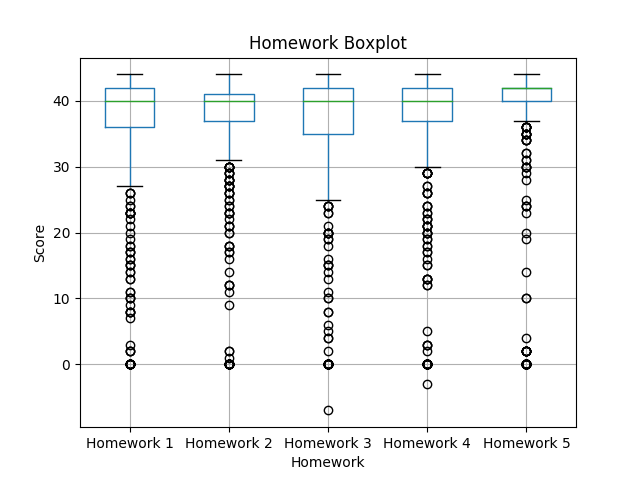
\includegraphics[scale=.7]{images/hwbox.png}
    \caption{Homework Boxplot}
\end{figure}
\begin{flushleft}
Figure 1 shows box plots for Homework 1 - 5 throughout all the semesters. The Box plot shows the minimum, 25\% quartile, the median, 75\% quartile and the maximum of the dataset, as well as outliers drawn as circles. From the plot, we could see that the means for all homework are mostly around 40, where as the sparsity of homework 1 and 3 are much greater than that of homework 5, indicating that homework 5 might have an easier set of questions comparing to the others.
\end{flushleft}
\begin{figure}[h]
    \centering
    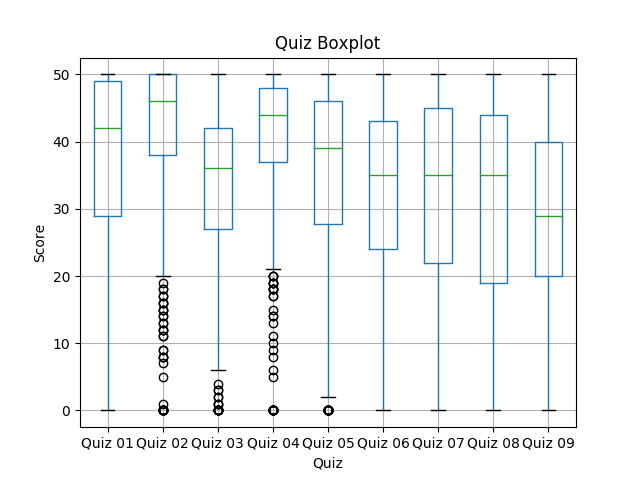
\includegraphics[scale=.7]{images/quizbox.png}
    \caption{Quiz Boxplot}
\end{figure}
\begin{flushleft}
Figure 2 shows box plots for Quiz 1 - 9 through all the semesters. The boxes of quizzes 1 and 2 indicate that students mostly have a higher score on these two quizzes compared to the others, and the line under the boxes of quiz 6 - 9 indicates that there are more people in the lower range for these quizzes, showing that possibly those quizzes are more difficult.
\end{flushleft}
\begin{figure}[h]
    \centering
    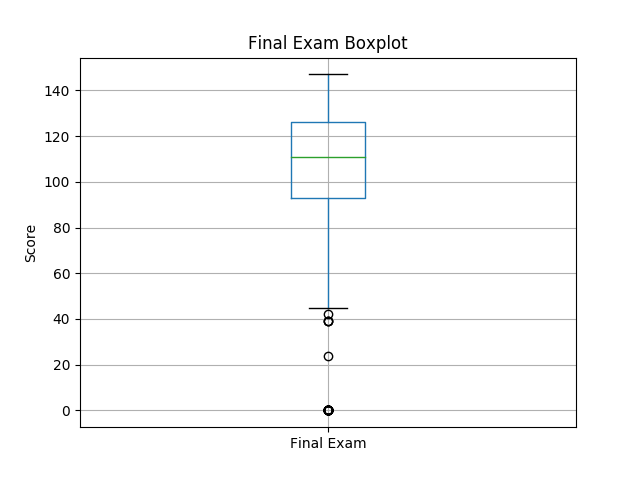
\includegraphics[scale=.6]{images/finalbox.png}
    \caption{Final Exam Boxplot}
\end{figure}
\begin{flushleft}
Figure 3 shows the box plot for the final exam. From the plot, we could tell that the median is around 110 marks and most students got marks between 95 and 125.
\end{flushleft}
\newpage
\begin{figure}[h]
    \centering
    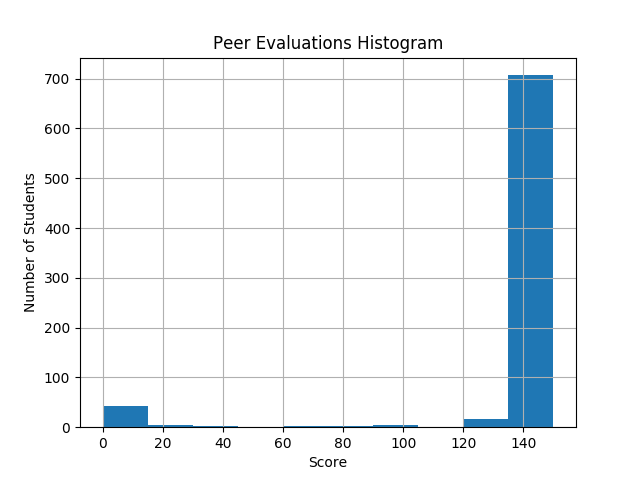
\includegraphics[scale=.5]{images/pehist.png}
    \caption{Peer Evaluations Histogram}
\end{figure}
\begin{flushleft}
Figure 4 is a histogram for Peer Evaluation scores. Histogram shows the overall distribution of a data set in a straightforward manner. From Figure 4, we could see that almost everyone got around 140 marks, very few between 120 - 135 and from 0 to 15.
\end{flushleft}
\begin{figure}[h]
    \centering
    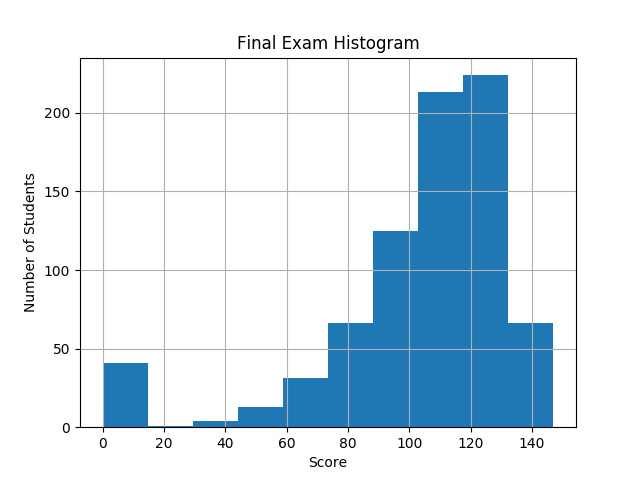
\includegraphics[scale=.5]{images/finalhist.png}
    \caption{Final Exam Histogram}
\end{figure}
\begin{flushleft}
Figure 5 is a histogram for the Final Exam scores. From the figure, we notice that most students has got scores around 100 - 130, others mostly got between 60 - 100 and 130 - 150. Very few got other marks.
\end{flushleft}
\begin{figure}[h]
    \centering
    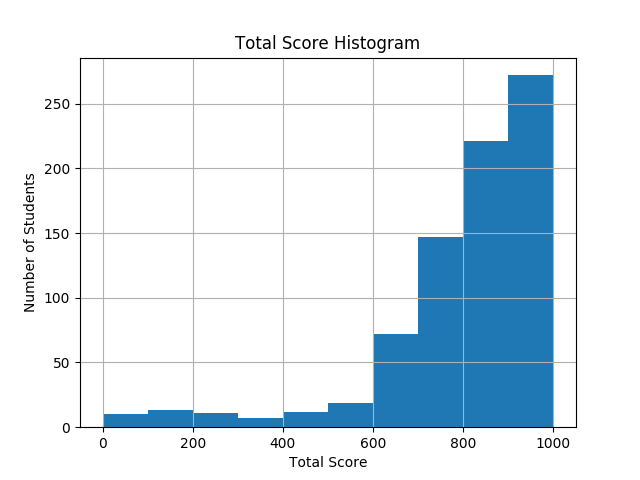
\includegraphics[scale=.5]{images/totalhist.png}
    \caption{Total Score Histogram}
\end{figure}
\begin{flushleft}
Figure 6 is a histogram for the Total scores. The figure shows that most students got 800 - 1000 marks, fewer got 600 - 800 marks, and very few got 0 - 600 marks.
\end{flushleft}
\begin{figure}[h]
    \centering
    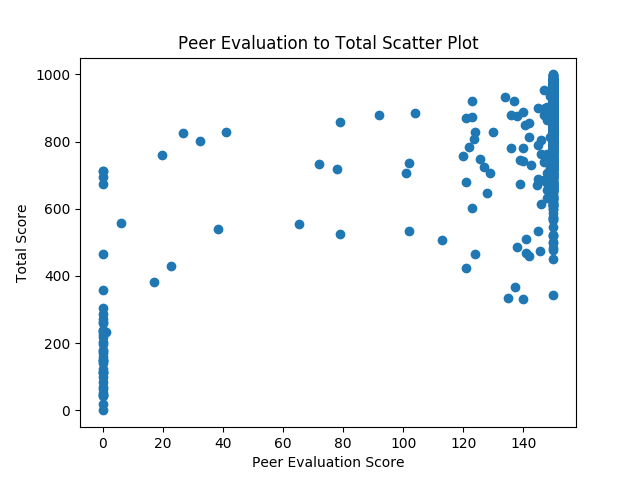
\includegraphics[scale=.7]{images/pescat.png}
    \caption{Peer Evaluations vs Total Score Scatter Plot}
\end{figure}
\begin{flushleft}
Figure 7 is a scattered plot that shows correlation between two attributes. In this case, Peer Evaluation Scores and Total Scores. From the graph, we could see there are clusters on the very left edge and very right edge. It does tell us that students with high peer evaluation scores also have pretty high total scores, and people with low or 0 peer evaluation scores have very low total scores as well.
\end{flushleft}
\begin{figure}[h]
    \centering
    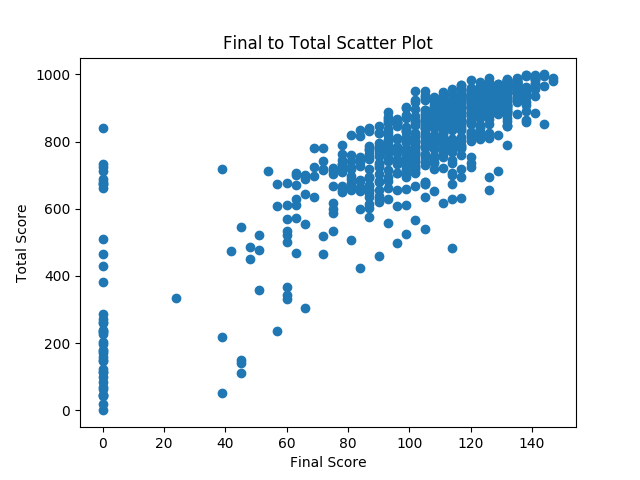
\includegraphics[scale=.6]{images/finalscat.png}
    \caption{Final Exam vs Total Score Scatter Plot}
\end{figure}
\clearpage
\begin{flushleft}
From Figure 8, we could see a nearly diagonal shape that clusters on the upper right section of the graph. The approximation to a straight line indicates that there is indeed a positive relation between the final exam scores and the total score.
\end{flushleft}
\begin{figure}[h]
    \centering
    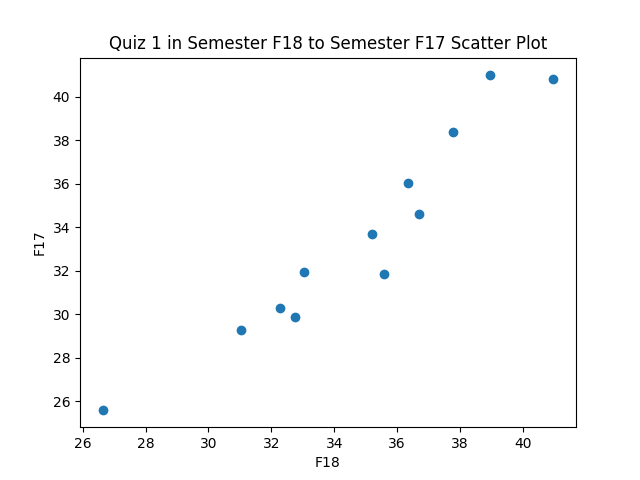
\includegraphics[scale=.6]{images/quizMeanSemScat.png}
    \caption{Quiz 1 Semester F18 vs F17 Scatter Plot}
\end{figure}
\begin{flushleft}
Figure 9 also shows a positive correlation between Quiz 1 scores in Semester F18 and F17. Their slope also looks very similar to each other. This indicates that the difficulty and the students' capabilities are very similar in the two semesters.
\end{flushleft}
\begin{figure}[h]
    \centering
    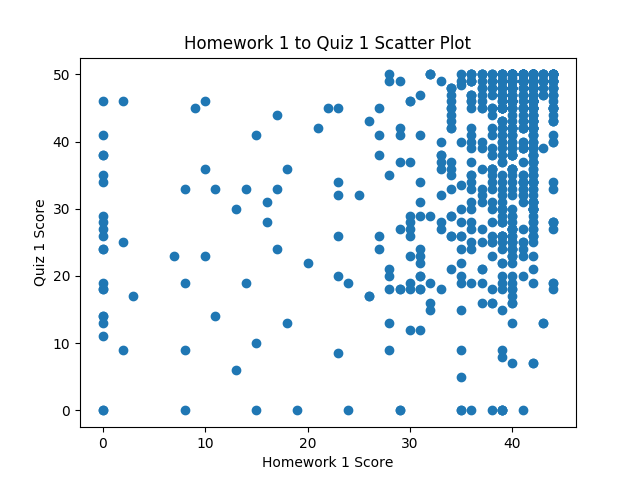
\includegraphics[scale=.6]{images/hw1quiz1scat.png}
    \caption{Homework 1 vs Quiz 1 Scatter Plot}
\end{figure}
\noindent
\justifying
From Figure 10, we could see the dots are scattered all over the graph, except on the top right corner, where there is obviously a cluster formed. This indicates that students with high Homework 1 Score usually have high score on Quiz 1 as well.

\section{Tools and languages}
For this homework, I have used Python Pandas, NumPy, and Matplotlib modules for data manipulation, and excel for viewing the dataframe. \\\\
Pandas is a python module for data analysis and manipulation, and it is good for dealing with large number of data, and it is very flexible and customizable. Numpy is a python module that provides embedding calculation methods for large number of data. In this case, it calculates the Mean, Standard Deviation and other statistics very quickly for the column attributes. Matplotlib creates the plots for data visualization. You can plot basically any graph you want, with customized fonts, colors, text sizes and so on, and you can plot several graphs combined in one. \\\\
However, although these tools are good for large number of data manipulation, it is usually not easy to find a single row, attribute with several conditions when the data frame is not too large. For example, if I want to find the name of the first person with missing Peer Evaluations score, I would need to set several conditions in python, while I just need to scan through the table if I'm working on Excel. \\\\
Excel, on the other hand, provides better visualization of the data frame. Firstly, you can access the data that you want as soon as you see it. You don't have to program anything if the data frame is not that big, and it's easy to find the data you want. Secondly, you can look at the data as you insert or update it. The instantaneous feedback could let you know right away whether your change is correct. Moreover, the Excel UI saves you a lot of time from reading documentation for python's modules.

\section{Code used for data manipulation}
\lstinputlisting[language=Python]{hw1.py}
\end{document}
